\begin{subfigure}[b]{.3\textwidth}
  \centering
  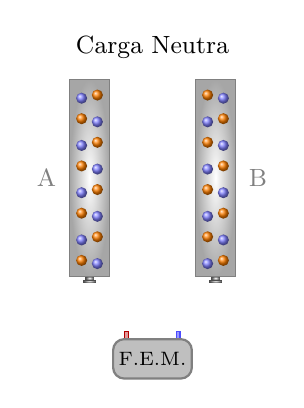
\begin{tikzpicture}
    \shade[inner color=white,outer color=black!70] (-.85,0) rectangle (-.75,-.05);
    \shade[inner color=white,outer color=black!70] (-.88,-.05) rectangle (-.72,-.08);

    \shade[inner color=white,outer color=black!70] (.85,0) rectangle (.75,-.05);
    \shade[inner color=white,outer color=black!70] (.88,-.05) rectangle (.72,-.08);

    \shadedraw[inner color=white,outer color=gray!70,color=gray] (-1.05,0) rectangle node[left=3mm] {\small A} (-0.55,2.5);
    \shadedraw[inner color=white,outer color=gray!70,color=gray] (1.05,0) rectangle node[right=3mm] {\small B} (0.55,2.5);
    \node at (0,2.9) {\small Carga Neutra};

    \filldraw[color=red!70!black,fill=red!70!black!40] (-.35,-.8) rectangle (-.3,-0.7);
    \filldraw[color=blue!70,fill=blue!40] (.35,-.8) rectangle (.3,-0.7);
    \filldraw[thick,color=gray,fill=gray!50,rounded corners] (-.5,-1.3) rectangle node {\color{black}\scriptsize F.E.M.} (.5,-0.8);

    \foreach \x\y in {.7/2.3,.9/2,.7/1.7,.9/1.4,.7/1.1,.9/.8,.7/.5,.9/.2} {
      \shade[ball color=orange] (\x,\y) circle (2pt);
      \shade[ball color=orange] (-\x,\y) circle (2pt);
    }

    \foreach \x\y in {.9/2.26,.7/1.96,.9/1.66,.7/1.36,.9/1.06,.7/.76,.9/.46,.7/.16} {
      \shade[ball color=blue!50] (\x,\y) circle (2pt);
      \shade[ball color=blue!50] (-\x,\y) circle (2pt);
    }
  \end{tikzpicture}
\end{subfigure}
\hfill 
\begin{subfigure}[b]{.3\textwidth}
  \centering
  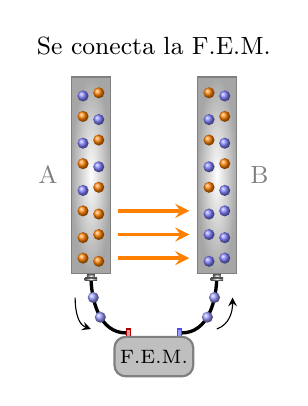
\begin{tikzpicture}[>=stealth]
    \draw[very thick] (-.8,0) to[out=270,in=180] (-.35,-.75);
    \shade[inner color=white,outer color=black!70] (-.85,0) rectangle (-.75,-.05);
    \shade[inner color=white,outer color=black!70] (-.88,-.05) rectangle (-.72,-.08);

    \draw[very thick] (.8,0) to[out=270,in=0] (.35,-.75);
    \shade[inner color=white,outer color=black!70] (.85,0) rectangle (.75,-.05);
    \shade[inner color=white,outer color=black!70] (.88,-.05) rectangle (.72,-.08);

    \draw[->] (-1,-.3) to[out=270,in=160] (-.8,-.7);
    \draw[<-] (1,-.3) to[out=270,in=20] (.8,-.7);
  
    \foreach \x\y in {.77/-.3,.68/-.55} {
      \shade[ball color=blue!40] (\x,\y) circle (2pt);
      \shade[ball color=blue!40] (-\x,\y) circle (2pt);
    }

    \shadedraw[inner color=white,outer color=gray!70,color=gray] (-1.05,0) rectangle node[left=3mm] {\small A} (-0.55,2.5);
    \shadedraw[inner color=white,outer color=gray!70,color=gray] (1.05,0) rectangle node[right=3mm] {\small B} (0.55,2.5);
    \node at (0,2.9) {\small Se conecta la F.E.M.};

    \filldraw[color=red!70!black,fill=red!70!black!40] (-.35,-.8) rectangle (-.3,-0.7);
    \filldraw[color=blue!70,fill=blue!40] (.35,-.8) rectangle (.3,-0.7);
    \filldraw[thick,color=gray,fill=gray!50,rounded corners] (-.5,-1.3) rectangle node {\color{black}\scriptsize F.E.M.} (.5,-0.8);

    \foreach \x\y in {.7/2.3,.9/2,.7/1.7,.9/1.4,.7/1.1} {
      \shade[ball color=orange] (\x,\y) circle (2pt);
      \shade[ball color=orange] (-\x,\y) circle (2pt);
    }
    \foreach \x\y in {.9/.8,.7/.5,.9/.2} {
      \shade[ball color=blue!50] (\x,\y) circle (2pt);
      \shade[ball color=orange] (-\x,\y) circle (2pt);
    }

    \foreach \x\y in {.9/2.26,.7/1.96,.9/1.66,.7/1.36,.9/1.06} {
      \shade[ball color=blue!50] (\x,\y) circle (2pt);
      \shade[ball color=blue!50] (-\x,\y) circle (2pt);
    }
    \foreach \x\y in {.7/.76,.9/.46,.7/.16} {
      \shade[ball color=blue!50] (\x,\y) circle (2pt);
      \shade[ball color=orange] (-\x,\y) circle (2pt);
    }
    \foreach \y in {.2,.5,.8} {
      \draw[very thick,orange,->] (-.45,\y) -- (.45,\y);
    }
  \end{tikzpicture}
\end{subfigure}
\hfill 
\begin{subfigure}[b]{.3\textwidth}
  \centering
  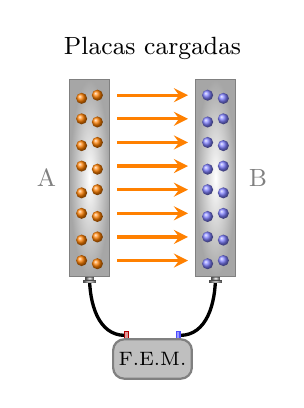
\begin{tikzpicture}[>=stealth]
    \draw[very thick] (-.8,0) to[out=270,in=180] (-.35,-.75);
    \shade[inner color=white,outer color=black!70] (-.85,0) rectangle (-.75,-.05);
    \shade[inner color=white,outer color=black!70] (-.88,-.05) rectangle (-.72,-.08);

    \draw[very thick] (.8,0) to[out=270,in=0] (.35,-.75);
    \shade[inner color=white,outer color=black!70] (.85,0) rectangle (.75,-.05);
    \shade[inner color=white,outer color=black!70] (.88,-.05) rectangle (.72,-.08);

    \shadedraw[inner color=white,outer color=gray!70,color=gray] (-1.05,0) rectangle node[left=3mm] {\small A} (-0.55,2.5);
    \shadedraw[inner color=white,outer color=gray!70,color=gray] (1.05,0) rectangle node[right=3mm] {\small B} (0.55,2.5);
    \node at (0,2.9) {\small Placas cargadas};

    \filldraw[color=red!70!black,fill=red!70!black!40] (-.35,-.8) rectangle (-.3,-0.7);
    \filldraw[color=blue!70,fill=blue!40] (.35,-.8) rectangle (.3,-0.7);
    \filldraw[thick,color=gray,fill=gray!50,rounded corners] (-.5,-1.3) rectangle node {\color{black}\scriptsize F.E.M.} (.5,-0.8);

    \foreach \x\y in {.7/2.3,.9/2,.7/1.7,.9/1.4,.7/1.1,.9/.8,.7/.5,.9/.2} {
      \shade[ball color=blue!50] (\x,\y) circle (2pt);
      \shade[ball color=orange] (-\x,\y) circle (2pt);
    }

    \foreach \x\y in {.9/2.26,.7/1.96,.9/1.66,.7/1.36,.9/1.06,.7/.76,.9/.46,.7/.16} {
      \shade[ball color=blue!50] (\x,\y) circle (2pt);
      \shade[ball color=orange] (-\x,\y) circle (2pt);
    }

    \foreach \y in {.2,.5,...,2.6} {
      \draw[very thick,orange,->] (-.45,\y) -- (.45,\y);
    }
  \end{tikzpicture}
\end{subfigure}
